\documentclass[xcolor=dvipsnames]{beamer}

\usepackage[utf8]{inputenc}
\usepackage[portuguese]{babel}
\usepackage[T1]{fontenc}
\usepackage{amsmath}
\usepackage{indentfirst}
\usepackage{amsfonts}
\usepackage{amssymb}
\usepackage{graphicx}
\usepackage{tikz}
%\usepackage{axodraw2}
\usepackage{subcaption}

% Uso de uma fonte especial que eu acho bonite
\usepackage{fourier}

\usetikzlibrary{3d}
\DeclareMathOperator*{\sen}{sen}
\renewcommand{\vec}{\mathbf}

\usetheme{Madrid}

\definecolor{azulUFPel}{rgb}{0.0, 0.25, 0.55}
\usecolortheme[named=azulUFPel]{structure}
\usefonttheme{serif}

% Uns trecos que eu fiz pra ficar mais ao meu gosto estético
\setbeamertemplate{itemize item}[triangle]
\setbeamertemplate{enumerate item}[square]
\setbeamertemplate{navigation symbols}{}
\setbeamertemplate{section in toc}[square]

\title{Método dos Fótons Equivalentes}
\subtitle{Revisão e Aplicações}
\author[A. A. S. Pacheco]{
	Alfredo Achterberg S. Pacheco\\
	{\footnotesize Orientado por: Prof.  Dr. Werner Krambeck Sauter}
}
\institute[IFM - UFPel]{
	Instituto de Física e Matemática - Universidade Federal de Pelotas
}
\date[25 de set., 2023]{25 de Setembro, 2023}
\titlegraphic{
	
\includegraphics[height=1.5cm]{
		./logos/logoUFPEL.png
	}
	\hspace{1cm}
	
\includegraphics[height=1cm]{
		./logos/logoFNDE.png
	}
	\hspace{1cm}
	
\includegraphics[height=1cm]{
		./logos/ifm_logo.png
	}
}
%\logo{
\includegraphics[width=0.15\textwidth]{logoUFPel.png}}

\begin{document}

\frame{\titlepage}

\begin{frame}
\frametitle{Estrutura da Apresentação}
\tableofcontents
\end{frame}

\section{Introdução e Contextualização}

\begin{frame}
	\frametitle{Introdução e Contextualização}

	\begin{columns}
	\column{0.5\textwidth}	
		\begin{figure}
			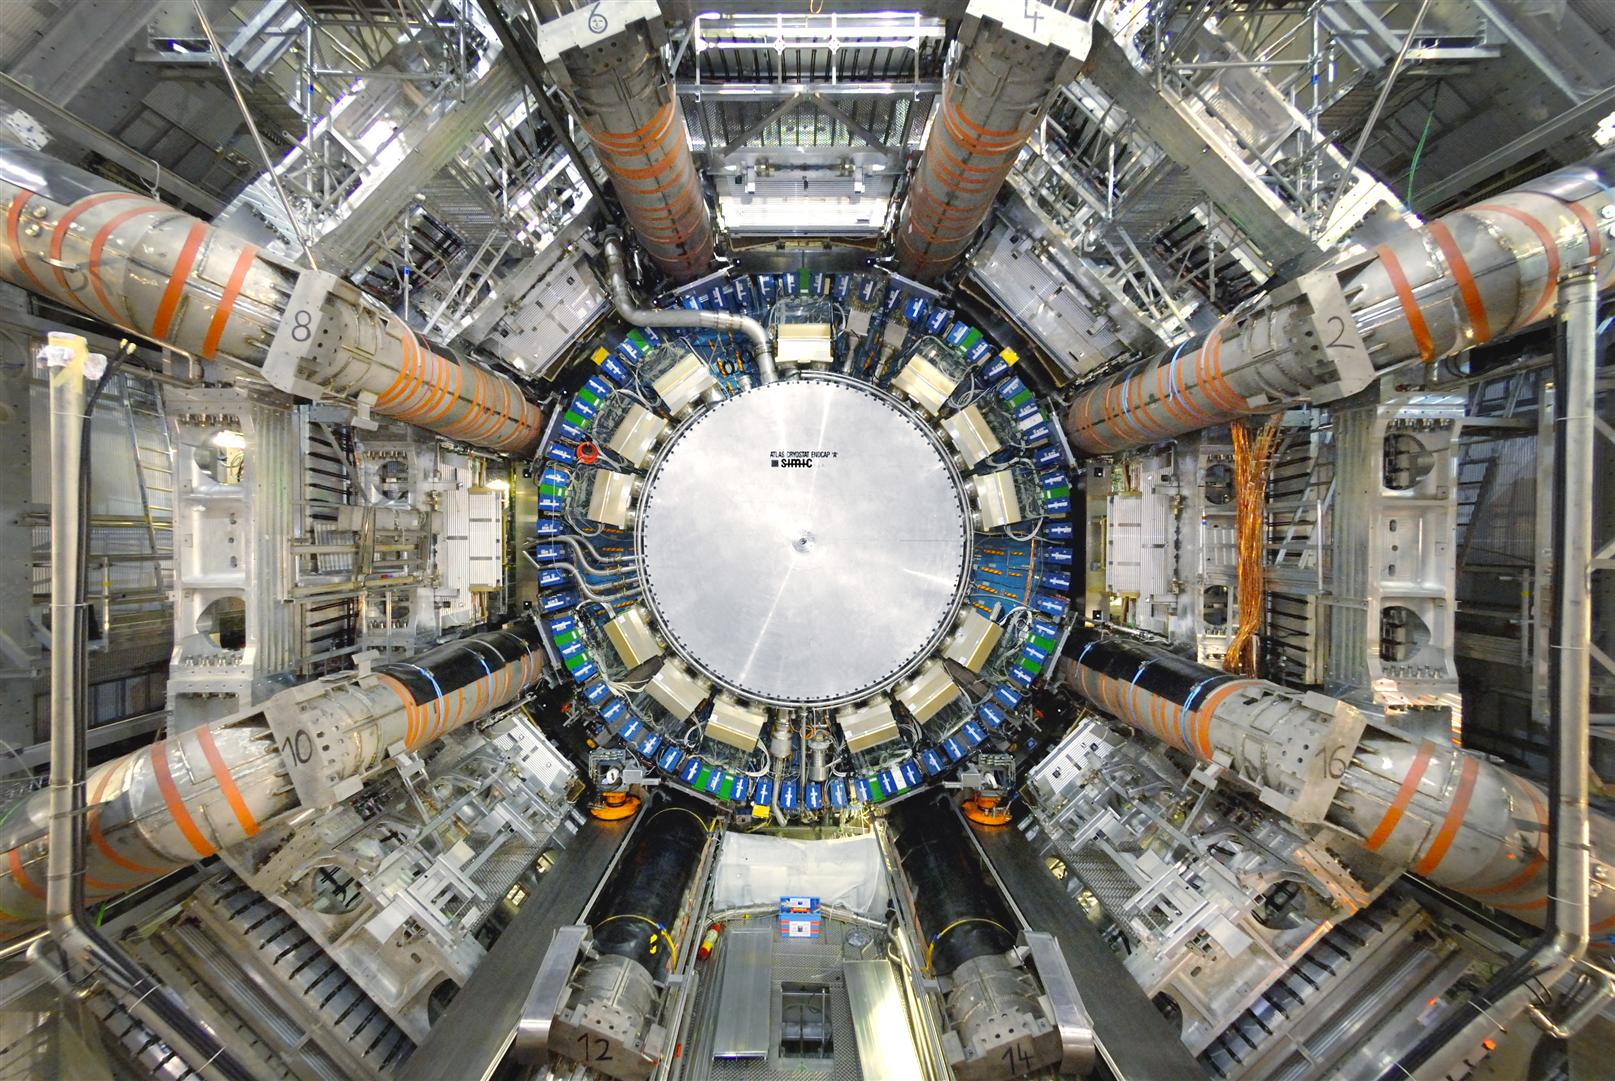
\includegraphics[width=\columnwidth]{./figs/atlan_normal.jpg}
			\caption{Foto do detector ATLAS do LHC. {\scriptsize Créditos:
			[\url{https://home.web.cern.ch/science/experiments/atlas}]}}
		\end{figure}
	
	\column{0.5\textwidth}
		Colisões de partículas constituem o método experimental mais utilizado
		atualmente para o entendimento da estrutura fundamental da matéria e de
		teste para novos modelos físicos.
	\end{columns}

\end{frame}

\begin{frame}
	\frametitle{Introdução e Contextualização}
	Estudos desse tipo de processo tem longa história na física.
	\begin{itemize}
		\item Como exemplo o trabalho de decréscimo de velocidade de partículas
			$\alpha$ e $\beta$ em meios materiais por N. Bohr;
		\item nesse trabalho, o físico propôs que a interação de partículas
			carregadas pode ser entendida pelo fenômeno eletromagnético de
			dispersão (uma analogia);
		\item em 1924, E. Fermi propôs que os campos de uma partícula carregada
			podem ser aproximados como pulsos de onda ou \textit{fluxos de
			fótons virtuais.}
	\end{itemize}
\end{frame}

\begin{frame}
	\frametitle{Introdução e Contextualização}

	\begin{columns}
	\column{0.6\textwidth}

	Disso, E. J. Williams, em 1933, propôs a generalização relativística do que
	seria o método dos fótons equivalentes.
	\begin{itemize}
		\item O método consiste, de forma introdutória, em obter o número de 
			fótons virtuais do campo eletromagnético de uma partícula a
			partir da transformada de Fourier dos mesmos campos;
		\item este consiste de uma aproximação \textit{semi-clássica} para
			o cálculo desses fótons virtuais.
	\end{itemize}

	\column{0.4\textwidth}

	\begin{figure}
	\begin{tikzpicture}[thick]
		\draw(-2,2) ellipse (0.15 and 0.75);
		\draw(0,0) ellipse (0.15 and 0.75);
		\node[left] (z1) at (-2.15,2) {$Z_1e$};
		\node[right] (z2) at (0.15,0) {$Z_2 e$};

		\draw[->](-2,2.75) -- (-2,3.75);
		\draw[->, rotate around={15:(-2,2.75)}](-2,2.75) -- (-2,3.75);
		\draw[->, rotate around={-15:(-2,2.75)}](-2,2.75) -- (-2,3.75)
			node[right]{$\vec{E}$};

		\draw[->](-2,1.25) -- (-2,0.25);
		\draw[->, rotate around={15:(-2,1.25)}](-2,1.25) -- (-2,0.25);
		\draw[->, rotate around={-15:(-2,1.25)}](-2,1.25) -- (-2,0.25);

		\draw[->](0,0.75) -- (0,1.75);
		\draw[->, rotate around={15:(0,0.75)}](0,0.75) -- (0,1.75);
		\draw[thick, ->, rotate around={-15:(0,0.75)}](0,0.75) -- (0,1.75);

		\draw[->](0,-0.75) -- (0,-1.75);
		\draw[->, rotate around={15:(0,-0.75)}](0,-0.75) -- (0,-1.75);
		\draw[->, rotate around={-15:(0,-0.75)}](0,-0.75) -- (0,-1.75);

		\draw[->](-1.85,2) -- (-1,2);
		\draw[->](-0.15,0) -- (-1.15,0) node[below]{$v \approx c$};
	\end{tikzpicture}
	\caption{Esquema representando os campos relativísticos de dois íons $Z_1$
		e $Z_2$.}
	\end{figure}


	\end{columns}
\end{frame}

\begin{frame}
	\frametitle{Introdução e Contextualização}

	Desde tais desenvolvimentos, este método aproximativo teve maior aplicação e
	desenvolvimentos na área de interação nuclear e de partículas fundamentais.

	\begin{itemize}
		\item Em especial, focaremos nas colisões ultraperiféricas de íons;
		\item são colisões com maior distância (parâmetro de impacto) e com
			interação dominantemente eletromagnética;
		\item pela interação ser eletromagnética também há menos multiplicidade
			nos estados finais e os resultados experimentais são mais facilmente
			tratados;
		\item fenômenos de interesse nesses processos incluem a produção de
			pares de partículas a partir de colisões de fótons.
	\end{itemize}
\end{frame}

\section{Objetivos do Trabalho}
\begin{frame}
	\frametitle{Objetivos do Trabalho}

	Para a realização do trabalho propomos uma revisão bibliográfica com cálculo
	analítico e computacional de quantidades de interesse dos processos de
	colisão. Para isso, temos os seguintes objetivos específicos:

	\begin{enumerate}
		\item realizar a revisão bibliográfica do método;
		\item realizar o cálculo do fator de forma para o fator de forma
			para diferentes distribuições de carga;
		\item deduzir o número de fótons equivalentes para diferentes
			distribuições de carga;
		\item realizar um estudo mais aprofundado sobre o fenômeno de
			fotoprodução de pares de partícula-antipartícula;
		\item obter as curvas teóricas para as seções de choque de diferentes
			processos de colisão e compará-las com as curvas experimentais.
	\end{enumerate}

\end{frame}

\section{Seção de Choque Diferencial e Total}
\begin{frame}
	\frametitle{Seção de Choque Diferencial e Total}

	O problema de interesse do método é o de colisão de partículas carregadas.
	A quantidade de interesse em colisões é a seção de choque.

	\begin{figure}[h]
		\centering
		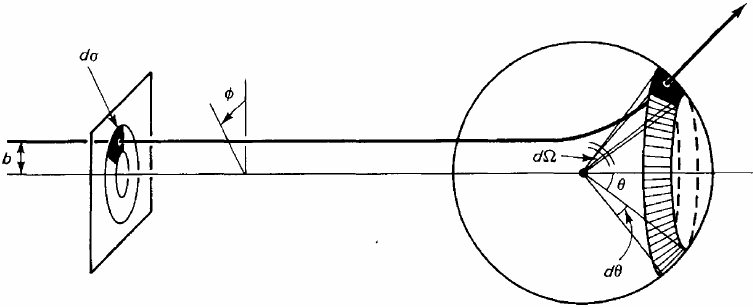
\includegraphics[width=0.8\textwidth]{./figs/cross_section.jpeg}
		\label{fig_cross_section}
		\caption{Partícula adentrando a região de espalhamento por uma
		seção de área $d\sigma$ e  sendo espalhada em um ângulo sólido
		$d\Omega$.}
	\end{figure}
\end{frame}

\begin{frame}
	\frametitle{Seção de Choque Diferencial e Total}

	\begin{columns}
	\column{0.5\textwidth}
	Da figura temos as diferenciais,
	\begin{gather}
		d\sigma = |b\, db\, d\phi|,\\
		d\Omega = |\sen \theta \, d\theta \, d\phi|.
	\end{gather}
	A razão entre as duas é,
	\begin{equation}
		\frac{d\sigma}{d\Omega} = \bigg| \frac{b}{\sen \theta}
		\frac{db}{d\theta} \bigg|. \label{diff_cross_section}
	\end{equation}
	Que é a seção de choque diferencial.

	\column{0.5\textwidth}
	A seção de choque total vem pela integral sobre $\Omega$,
	\begin{equation}
		\sigma = \int \frac{d\sigma}{d\Omega} \sen \theta \, d\theta \, d\phi .
	\end{equation}

	\end{columns}

\end{frame}

\begin{frame}
	\frametitle{Seção de Choque Diferencial e Total}
	\begin{block}{Isto para uma partícula incidente individual!}
		Estamos levando em conta uma partícula individual. Se quisermos tratar
		um feixe de partículas, vamos precisar definir a \textit{luminosidade}.
	\end{block}

\end{frame}

\begin{frame}
	\frametitle{Seção de Choque Diferencial e Total}
	\begin{block}{Luminosidade}
		Para um feixe de $N$ partículas com mesma energia atravessando a área
		$d\sigma$, a luminosidade $\mathcal{L}$ é definida como a quantidade
		de partículas que atravessam a região de espalhamento por unidade de
		área por unidade de tempo.
	\end{block}
	Disso, reescrevemos a seção de choque para um feixe de múltiplas partículas,
	\begin{gather}
		dN = \mathcal{L} d\sigma, \\
		\Rightarrow \frac{d\sigma}{d\Omega} = \frac{1}{\mathcal{L}}
		\frac{dN}{d\Omega}.
	\end{gather}
\end{frame}

\section{Demonstração do Método para Partícula Incidente Pontual}
\begin{frame}
	\frametitle{Demonstração do Método para Carga Pontual}
	A dedução do método segue os seguintes passos:
	\begin{itemize}
		\item obter os campos de uma carga pontual em movimento pela
			transformada de Lorentz;
		\item calcular a transformada de Fourier para a frequência dos campos,
			obtendo assim o espectro de frequência;
		\item a quantização do espectro de frequência nos fornece o número de
			fótons equivalentes dos campos da partícula.
	\end{itemize}
\end{frame}

\begin{frame}
	\frametitle{Demonstração do Método para Carga Pontual}
	Inicialmente consideramos uma carga em movimento como abaixo.\footnote{A partir daqui usaremos unidades naturais ($\hslash = c = 1$).}
	\begin{figure}
		\begin{tikzpicture}[thick, scale=0.65]
		% A caceta dos eixos...
			\draw[-] (0,0) --  (13,0)node[below right]{$x_1$};
			\draw[-] (0,0) -- (0,4) node[above]{$x_2$};
			\draw[-] (0,0) -- (0,0,3) node[below left]{$x_3$};
			\draw[-] (5,0.4) -- (13.5,0.4) node[right]{$x'_1$};
			\draw[-] (5,0.4) -- (5,4) node[above]{$x' _2$};
			\draw[-] (5,0.4) -- (5,0.2,3) node[below left]{$x'_3$};

		% A caceta dos desenhos que importam
			\filldraw (5,0.4) circle(3pt) node[above right] {$q$};
			\filldraw (0,3) circle(3pt) node[above right] {$P$};
			\draw (0,3) -- node[above]{$r$} (5,0.4);
			\draw[|-|,dashed] (-0.3,0) -- node[fill=white,left]{$b$} (-0.3,3);
			\draw[->,ultra thick] (5,0.4) -- (7,0.4) node[above]{$\vec{v}$};
	\end{tikzpicture}
	\caption{Carga $q$ em movimento com velocidade $\vec{v}$ passando por um
		ponto de observação $P$ com parâmetro de impacto $b$ e distância $r$.}
	\end{figure}
\end{frame}

\begin{frame}
	\frametitle{Demonstração do Método para Carga Pontual}
	Sendo os campos elétrico e magnético escritos em termos dos potenciais,
	\begin{gather}
		\vec{E} = - \nabla \Phi - \frac{\partial \vec{A}}{\partial t}, \\
		\vec{B} = \nabla \times \vec{A},
	\end{gather}
	estes são escritos em forma explicitamente covariante usando o tensor
	eletromagnético,
	\begin{equation}
		(F^{\mu \nu}) = \begin{pmatrix}
			0 & -E_1 & -E_2 & -E_3 \\
			E_1 & 0 & -B_3 & B_2 \\
			E_2 & B_3 & 0 & -B_1 \\
			E_3 & -B_2 & B_1 & 0
		\end{pmatrix}.
	\end{equation}
\end{frame}

\begin{frame}
	\frametitle{Demonstração do Método para Carga Pontual}
	Este se transforma como, 
	\begin{equation}
		{F'}^{\mu \nu} = \Lambda _\alpha ^\mu \Lambda _\beta ^\nu F^{\alpha
		\beta}
	\end{equation}
	onde $\Lambda _\mu ^\nu$ são os componentes da matriz de transformação
	de Lorentz,
	\begin{equation}
		(\Lambda ^\mu _\nu) = \begin{pmatrix}
			\gamma & -\gamma \beta & 0 & 0 \\
			-\gamma \beta & \gamma & 0 & 0 \\
			0 & 0 & 1 & 0 \\
			0 & 0 & 0 & 1
		\end{pmatrix},
	\end{equation}
	sendo $\gamma = (1-\beta ^2)^{-1/2}$ e $\beta = v/c$ os parâmetros
	relativísticos da partícula.
\end{frame}

\begin{frame}
	\frametitle{Demonstração do Método para Carga Pontual}
	A transformação dos campos é assim obtida como,
	\begin{equation}
		\label{eq_field_trans}
		\begin{cases}
		E_1' = E_1 \\
		E_2' = \gamma (E_2 - \beta B_3) \\
		E_3' = \gamma (E_3 + \beta B_2) \\
		\end{cases} \qquad
		\begin{cases}
		B_1 ' = B_1 \\
		B_2 ' = \gamma (B_2 + \beta E_3) \\
		B_3' = \gamma(B_3 - \beta E_2)
		\end{cases}.
	\end{equation}
\end{frame}


\section{Sobre o Fator de Forma}


\end{document}
